\begin{frame}[t]{Fibonacci}
	\par O método de Fibonacci é um método iterativo utilizado para localizar o mínimo de uma função. Esse método se baseia em intervalos simétricos que vão continuamente se reduzindo até uma determinada tolerância.
	
	\begin{figure}
		\centering
		\begin{minipage}{0.5\textwidth}
			\centering
			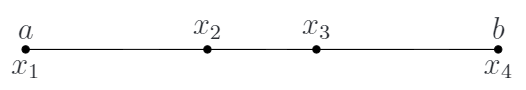
\includegraphics[width=5cm]{./fibonacci_ex1.png}
			\caption{Início do algoritmo}
			\label{}
		\end{minipage}\hfill
		\begin{minipage}{0.5\textwidth}
			\centering
			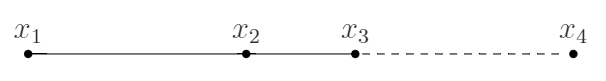
\includegraphics[width=5cm]{./fibonacci_ex2.png}
			\caption{Continuação do algoritmo}
			\label{}
		\end{minipage}
	\end{figure}
	
	 
\end{frame}

\begin{frame}[t]{Fibonacci}	
	\par Nesse caso podemos observar que $ f(x2)<f(x3) $, logo o novo intervalo se torna:
	
	\begin{figure}[h]
		\begin{center}
			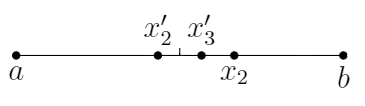
\includegraphics[width=6cm]{./fibonacci_ex3.png}    
			\caption{Fim do algoritmo}
			\label{fig:fibonacci_ex2}
		\end{center}
	\end{figure}
	
	\par Os pontos antigos são sempre reaproveitados!
	
\end{frame}